\chapter{原子核}
\section{天然放射现象}

\subsection{天然放射现象}

人类认识原子核的结构和它的变化规
律,是从发现天然放射现象开始的.

1896年,法国物理学家贝克勒耳(1852—1908)发现,铀和
含铀的矿物能发出某种看不见的射线,这种射线可以穿透黑
纸使照相底片感光.物质发射这种射线的性质,叫做\textbf{放射性};
具有放射性的元素,叫做\textbf{放射性元素}.

在贝克勒耳的建议下,玛丽·居里(1867—1934)和她的丈
夫皮埃尔·居里(1859—1906)对铀和铀的各种矿石进行了深
入的研究,并且发现了两种放射性更强的新元素,玛丽·居里
为了纪念她的祖国波兰,把其中一种元素命名为钋(读作“坡”,
元素符号是Po),另一种命名为镭.

放射性并不是少数几种元素才有的,实际上原子序数大
于83的所有天然存在的元素都具有放射性.这种能自发地
放出射线的现象叫做\textbf{天然放射现象}.

铀、钋和镭放出的射线到底是什么呢?科学家们利用电
场或磁场来研究放射线的性质,确定了放射线的组成.图9.1
表示利用电场进行研究的实验:把放射性样品放在铅块的窄
孔底上,在孔的对面放着照相底片,没有电场时,在显影后的
照相底片上可以发现正对着窄孔有一个暗斑,说明射线顺着
窄孔一直射到底片上,使它感光,在铅块和底片之间放上一
对电极,使电场的方向跟射线的方向垂直时,在显影后的底片
上出现三个暗斑,说明在电场作用下,射线分成三束(图9.1).
其中有两束向相反方向偏转,表明这两束射线是由带电粒子
组成的,而且两种粒子带有异种电荷;另外那束不发生偏转,
表明这束射线是中性的,从暗
斑的位置知道,带正电的射线
偏转较小,带负电的射线偏转
较大,通常把带正电的射线叫
做$\alpha$射线,带负电的射线叫做
$\beta$射线,不发生偏转的射线叫
做$\gamma$射线.

\begin{figure}[htp]
    \centering
    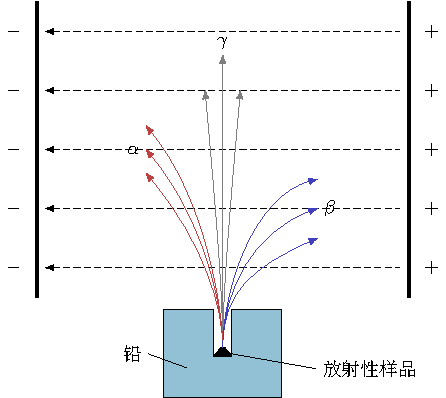
\includegraphics[scale=1.4]{fig/9-1.pdf}
    \caption{}
\end{figure}

卢瑟福对这些射线进一步研究,直接用实验证实$\alpha$粒子
带有两个单位的正电荷,质量数是4\footnote{在原子核物理中,把基本电荷取作电荷的单位;把碳原子质量
的1/12取作质量的单位,原子核的质量数通常非常接近整数,因此习
惯上都用整数表示.}.$\alpha$粒子就是氦原子核.
$\alpha$粒子射出时的速度约为光速的十分之一,$\alpha$射线贯穿物质
的本领很小,在空气中只能飞行几厘米,一张薄铝箔或一张薄
纸就能把它挡住;但是它有很强的电离作用,很容易使空气电
离,使照相底片感光的作用也很强.贝克勒耳用实验证实了$\beta$
射线是电子流,速度很接近光速.$\beta$射线的贯穿本领很大,很
容易穿透黑纸,甚至能穿透几毫米厚的铝板,但它的电离作用
比较弱.$\alpha$射线是一种波长很短的电磁波,它的贯穿本领最
强,甚至能穿透几厘米厚的铅板,但它的电离作用却很小.

这三种射线都是从原子核里放射出来的,实验指出,当
放射性物质连续发生衰变时,各种原子核中有的放射$\alpha$射线,
有的放射$\beta$射线,同时伴随,射线,这时在放射线中就会同时
有$\alpha$、$\beta$、$\gamma$三种射线,放射线的发现揭示了原子核结构的复
杂性,从而促进了人类对微观结构的认识.

\subsection{放射性元素的衰变}

某元素的原子核,例如铀核,放出一
个$\alpha$粒子后,就变成了新的原子核.我们把原子核由于放出
某种粒子而转变为新核的变化叫做原子核的衰变.在衰变中
电荷数和质量数都是守恒的,我们用$\atom{U}{238}{92}$代表铀原子核,上
标“238”表示核的质量数,下标“92”表示核的电荷数(可以省
去下标,简写为$\atom{U}{238}{}$,还可以简写为铀238或U238).同样
地,用$\atom{He}{4}{2}$代表氦原子核(即$\alpha$粒子),用$\atom{Th}{234}{90}$代表钍原子
核.于是,铀238核放出$\alpha$粒子变成钍234核的衰变可用下
面的方程来表示:
\[\atom{U}{238}{92}\longrightarrow \atom{Th}{234}{90}+\atom{He}{4}{2}\]
从这个方程可以看出,方程两边的质量数和电荷数都是相同
的.这种放出$\alpha$粒子的衰变叫做$\alpha$衰变.$\alpha$衰变的规律是:
新核的质量数比原来核的质量数减少4,新核的电荷数比原
来核的电荷数减少2,因此新核在元素周期表中的位置要向
前移两位,如果用$M$表示核的质量数,$Z$表示核的电荷数,则
$\alpha$衰变的规律可以用下式表示(式中$X$、$Y$表示不同元素):
\[\atom{X}{M}{Z}\longrightarrow \atom{Y}{M-4}{Z-2}+\atom{He}{4}{2}   \]

$\atom{U}{238}{92}$发生$\alpha$衰变产生的$\atom{Th}{234}{90}$也具有放射性,它能放出
一个$\beta$粒子而变成$\atom{Pa}{234}{91}$(镤).由于$\beta$粒子就是电子,电子的
质量比核的质量小得多,一个原子核放出一个$\beta$粒子后,它的
质量数不变,因此,可以认为电子的质量数是零,电荷数是$-1$,
于是我们用$\atom{e}{0}{-1}$来表示电子(即$\beta$粒子).上述的衰变可表示为:
\[\atom{Th}{234}{90}\longrightarrow \atom{Pa}{234}{91}+ \atom{e}{0}{-1}\]
这个方程两边的质量数和电荷数也是相同的,这种放出$\beta$粒
子的衰变叫做$\beta$衰变,$\beta$衰变的规律是:新核的质量数不变,
电荷数增加1,新核在元素周期表中的位置要向后移一位,$\beta$
衰变的规律可以用下式表示:
\[\atom{X}{M}{Z}\longrightarrow \atom{Y}{M}{Z+1}+ \atom{e}{0}{-1}\]



\subsection{半衰期}
放射性元素的衰变有一定的速率,例如,氡222
经过$\alpha$衰变变为钋218,如果隔一定时间测定一次剩余的氡的
数量,就会发现,大约每过3.8天,就有一半的氡发生了衰变.
也就是说,经过第一个3.8天以后,剩有一半的氡,经过第二
个3.8天以后,剩有四分之一的氡,再经过3.8天以后,就只剩
有八分之一的氡了.因此,我们可以用\textbf{半衰期}来表示放射性
元素衰变的速率:\textit{半衰期是放射性元素的原子核有半数发生
衰变需要的时间}.每一种放射性元素都有一定的半衰期,不
同的放射性元素,半衰期不同,甚至差别非常大.例如前面说
的氡222变为钋218的半衰期是3.8天,而镭226变为氡222
的半衰期是1620年,铀238变为钍234的半衰期竟长达$4.5
\x10^9$年!

放射性元素衰变的速率是由核内部本身的因素决定的,
而跟原子所处的物理状态或化学状态无关.例如,一种放射
性元素,不管它是成单质存在或是成化合物存在,或者对它施
加压力,或者增高它的温度,都不能改变它的半衰期.

\subsection*{练习一}
\begin{enumerate}
    \item 钍230是$\alpha$放射性的,它放出一个$\alpha$粒子后变成了
什么?写出衰变方程.
\item 钫223是$\beta$放射性的,它放出一个$\beta$粒子后变成了
什么?写出衰变方程.
\item 钍232经过六次$\alpha$衰变和四次$\beta$衰变后变成一种稳
定的元素.这种元素是什么?它的原子量是多少?它的原子序
数是多少?
\item 
$\atom{U}{238}{92}$变成$\atom{Pb}{206}{82}$,要经过几次$\alpha$衰变和几次$\beta$衰变?
\item 
$\atom{Bi}{210}{83}$的半衰期是5天.10克的铋210经过20天后
还剩下多少?
\item 放射性元素$\atom{Na}{24}{11}$经过6小时后只剩下1/8没有衰
变,它的半衰期是多少?
\end{enumerate}

\section{探测放射线的方法}
放射性元素放射出的$\alpha$射线、$\beta$射线和$\gamma$射线都是看不
见的,需要根据它们跟其他物质作用产生的各种效应,用适当
的仪器来探测,下面简单介绍三种方法.

\subsection{云室}
我们知道,水蒸气遇冷凝结,会形成很小的雾珠,
这时它需要有凝结的核心,悬浮在空气中的尘埃微粒或气体
离子都可以成为这种凝结核心.云和雾就是这样形成的.如
果空气中没有任何尘埃或离子,水蒸气就是达到过饱和状态,
也不能马上凝结.但是,如果这时由于某种原因在空气中产
生了离子,那么过饱和的水蒸气就会以这些离子为核心立即
凝结成雾珠.离子是看不见的,可是雾珠是看得见的,因此可
以根据出现的雾珠来推测产生离子的情形.云室就是根据这
个原理制成的.

\begin{figure}[htp]
    \centering
    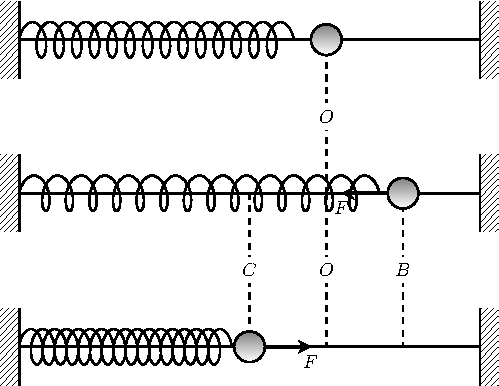
\includegraphics[scale=.35]{fig/9-2.pdf}
    \caption{云室}
\end{figure}

云室(图9.2)的主要部分是一个塑料或玻璃制的容器,
它的下底是在小范围内可以上下移动的活塞,上盖是透明的,
可以通过它来观察室内发生的现象或进行照相,一小块放射
性物质(放射源)放在室内侧壁附近(或放在室外,让放射线从
侧壁的窗射入).实验时,先往云室里加一些酒精或乙醚
(可以洒在云室下底上的黑绒布上),使室内充满酒精的饱和
蒸气,然后,使活塞突然迅速向下移动,室内气体由于迅速膨
胀而降低温度,于是酒精蒸气达到过饱和.这时如果有射线
粒子从室内气体中飞过,使沿途的气体分子电离,过饱和的酒
精蒸气就会以这些离子为核心凝结成一条雾迹,这种云室是
英国物理学家威耳逊(1869—1959)于1911年发明的,通常叫
做威耳逊云室.

\begin{figure}[htp]
    \centering
    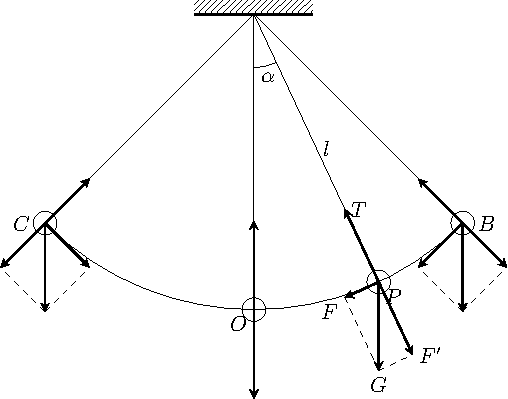
\includegraphics[scale=1.2]{fig/9-3.pdf}
    \caption{云室中的径迹}
\end{figure}

用云室可以清楚地看出$\alpha$粒子和$\beta$粒子的径迹(图9.3).
$\alpha$粒子质量较大,在气体中行进时不易改变方向,它的电离
本领大,在每厘米的路程中能使气体分子产生10000对离子,
所以它的径迹直而粗.$\beta$粒子质量很小,跟气体分子的电子
碰撞时容易改变方向,而且电离本领小,在每厘米的路程中只
能产生几百对离子,所以它的径迹比较细而且有时发生弯曲.
$\gamma$粒子电离本领更小,有时能产生一些细碎的雾迹.



\subsection{计数器}
\begin{figure}[htp]\centering
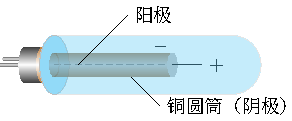
\includegraphics[scale=.6]{fig/9-4.png}
\caption{计数管}
\end{figure}

计数器的主要部分是计数管,它是一支玻璃管,
里面有一个导电的圆筒(或在管壁上涂一层导电薄膜)作阴
极,一根通过圆筒轴心的金属丝作阳极(图9.4),管里装入
惰性气体(如氩、氖等)和少量的乙醇汽或溴汽,气压大约是
$1.33\x10^4$—$2.66\x10^4$帕.在两极加上大约800—1500伏的直
流电压,这个电压略低于管内气体的击穿电压.当有射线粒子
飞进管内,使管内气体电离时,产生的电子在电场作用下向阳
极加速运动.电子在运动中能量越来越大,达到一定值时,跟
气体分子碰撞,又可使气体分子电离,再产生电子,于是经过
一段很短时间,就会产生大量电子,这些电子到达阳极,正离
子到达阴极(正离子由于质量大,运动较慢,在运动中不会再
使气体分子电离),就使计数管发生一次短暂的放电,从而得
到一个脉冲电流.这个脉冲电流可以用电子设备录下来.

这种计数器适合于对$\beta$粒子和$\gamma$粒子进行计数、$\alpha$粒
子的贯穿本领很小,要对它计数,需要在计数管上装一个很薄
的窗口,或者制成其他式样.

\subsection{乳胶照相}

放射线能够使照相底片感光,放射线中的粒
子经过照相底片上的乳胶时,使乳胶中的溴化银分解,经显影
后,就有一连串的黑点显示出粒子的径迹.这些径迹可用显
微镜来进行观察与测量,根据径迹的长短和形状,可以判断入
射粒子的性质、种类和能量.乳胶的密度较大,粒子在乳胶中
的射程约为空气中的千分之一,因此容易看到径迹的全部.乳
胶照相的主要优点是能够连续地工作,能够将入射粒子每个
时刻的径迹记录下来.

随着科学技术的发展,探测射线的手段不断改进,近年
来,由于探测仪器大都和电子计算机直接联结,实现了对实验
全过程电子计算机控制、计算、数据处理,已经使实验方法高
度自动化.

\section{原子核的人工转变~~原子核的组成}
放射现象的发现,使人们认识到原子核仍然具有内部结
构,并且是能够发生变化的,但是,能不能用人工的方法使原
子核发生变化呢?原子核是由什么组成的呢?

\subsection{质子的发现}
\begin{figure}[htp]\centering
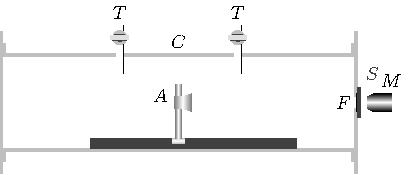
\includegraphics[scale=.75]{fig/9-5.png}
\caption{}
\end{figure}

1919年,卢瑟福做了用$\alpha$粒子轰击氮原子
核的实验.实验装置如图9.5所示.容器$C$里放有放射性物
质$A$,从$A$射出的$\alpha$粒子射到一个铝箔$F$上,适当选取铝箔
的厚度;使$\alpha$粒子恰好被它完全吸收,而不能透过,在$F$的后
面放一荧光屏$S$,用显微镜$M$来观察荧光屏上是否出现闪光.
通过阀门$T$往容器$C$里通入氮气后,卢瑟福从荧光屏$S$上观
察到了闪光,把氮气换成氧气或二氧化碳,又观察不到闪光.
这个实验表明,闪光一定是$\alpha$粒子击中氮核后产生的新粒子
透过铝箔引起的.

后来,把这种粒子引进电场和磁场中,根据它在电场和磁
场中的偏转,测出了它的质量和电量,确定它就是氢原子核,
又叫做\textbf{质子},通常用符号$\atom{H}{1}{1}$或$\atom{p}{1}{1}$表示.
\begin{figure}[htp]\centering
\begin{tikzpicture}[>=latex]
\draw [->](-1,-.5)node[above]{$\alpha$}--(-0.025,-0.025);
\draw [->](0,0)--node [below]{反冲核}(2,-.2);
\draw [->](0,0)--(.2,2)node[above]{$\alpha$};
\draw [->](0,0)--(1.25,1.25)node[below]{p};
\draw (0,0) [fill=gray] circle (2.5pt);
\node at (0,-1){甲};
\end{tikzpicture}\qquad\qquad \begin{tikzpicture}[>=latex]
    \draw [->](-1,-.5)node[above]{$\alpha$}--(-0.025,-0.025);
    \draw [->](0,0)--node [below]{反冲核}(2,-.2);    \draw [->](0,0)--(1.25,1.25)node[below]{p};
    \draw (0,0) [fill=gray] circle (2.5pt);
    \node at (0,-1){乙};

\end{tikzpicture}
\caption{}
\end{figure}

这个质子是$\alpha$粒子直接从氮核中打出的,还是$\alpha$粒子打
进氮核后形成的复核发生衰变时放出的呢?为了弄清这个问
题,英国物理学家布拉凯特又在充氮的云室里做了这个实验.
如果质子是$\alpha$粒子直接从氮核中打出的,那么在云室里就会
看到四条径迹:入射$\alpha$粒子的径迹,碰撞后$\alpha$粒子的径迹,质
子p的径迹,抛出质子后的核的反冲径迹(图9.6甲).如果
$\alpha$粒子打进氮核后形成一个复核,这复核立即发生衰变放出
一个质子,那么在云室里就只能看到三条径迹;入射$\alpha$粒子
的径迹,质子p的径迹,核的反冲径迹(图9.6乙),布拉凯特
拍摄了两万多张云室照片,终于从四十多万条$\alpha$粒子径迹的
照片中,发现有八条产生了分叉(图9.7),分叉的情况表明,
上述的第二种设想是正确的,从质量数守恒和电荷数守恒可
以知道,这个新核是质量数等于17的氧.这个变化过程可以
用下面的核反应方程来表示:
\[\atom{N}{14}{7}+\atom{He}{4}{2}\longrightarrow \atom{O}{17}{8}+\atom{H}{1}{1} \]
\begin{figure}[htp]\centering
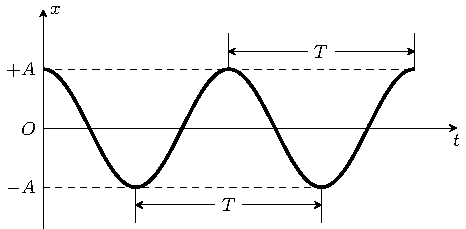
\includegraphics[scale=.75]{fig/9-7.png}
\caption{}
\end{figure}

在云室的照片中,分叉后细而长的是质子的径迹;短而粗
的是反冲氧核的径迹.

后来,人们用同样的方法使氟、钠、铝等核发生了类似的
转变,并且都产生了质子,由于从各种原子核里都能打出质
子来,可见质子是原子核的组成部分.

\subsection{中子的发现}

卢瑟福用$\alpha$粒子轰击氮核发现质子后,有
人提出原子核可能是由带正电的质子组成的.但这种设想遇
到的困难是:除了氢原子外,所有元素的原子核的电荷数并
不等于原子核的质量数,例如,氮核的质量数是4,电荷数是
2;铀238的质量数是238,电荷数是92.那么原子核里除了
质子外还有什么呢?

1920年,卢瑟福曾预言:可能有一种质量与质子相近的
不带电的中性粒子存在,他把它叫做\textbf{中子}.

1930年发现,用由钋放出的$\alpha$射线轰击铍(Be)时产生一
种射线,这种射线的贯穿能力极强,它能够穿透几厘米厚的
铅.当时,由被轰击物质产生的各种射线中,唯一能够贯穿铅
层的是$\gamma$射线,所以当时认为这种射线可能是$\gamma$射线.

1932年,约里奥·居里(1900—1958)和伊丽芙·居里(1897
—1956)夫妇发现,如果用来自铍的这种射线去轰击石蜡(含
有大量氢原子),竟能从石蜡中打出质子(图9.8).但从来也
没有发现过$\gamma$射线具有这样的性质,约里奥·居里夫妇想不
出这种射线是什么.
\begin{figure}[htp]\centering
\begin{tikzpicture}[>=latex] 
\draw (0,0) [fill=white] circle(2pt);
\foreach \x in{36,72,...,360}
{
    \draw[dashed,->](\x:.25)--(\x: 1);
}
\node at (0,.3){Po};
\node at (0,-1.2){$\alpha$-粒子};
\draw [pattern=north east lines] (1.3,-.3) rectangle (1.5,.3);
\node at (1.4,.6){Be};
\node at (3.4,.8){未知射线};

\foreach \x in{6,3,0,...,-6}
{
    \draw[dashed,->](\x:1.7)--(\x: 5);
}
\draw  (5.3,-.3) rectangle (5.5,.3);

\foreach \x in{6,3,0,...,-6}
{
    \draw[dashed,->](\x:1.7)--(\x: 5);
}

\draw [dashed,->] (5.6, 0)--(6.6, 0);
\draw [dashed,->] (5.6, 0.1)--(6.6, .3);
\draw [dashed,->] (5.6, -.1)--(6.6, -.3);
\node at (5.4,.6){石蜡};
\node at (6.1,-.6){质子};


\end{tikzpicture}
\caption{}
\end{figure}

1932年英国物理学家查德威克(1891—1974)仔细地研究
了这种射线,发现这种射线在磁场中不发生偏转,可见它是
中性粒子流.测出这种射线的速度不到光速的十分之一,因
此排除了它是$\gamma$射线的可能.查德威克用这种射线轰击氢原
子和氮原子.结果打出了一些氢核(质子)和氮核.他测量了
被打出的氢核和氮核的速度,并由此推算出这种射线粒子的
质量.

被打出的氢核的速度是不同的,查德威克认为速度最大
的氢核是由于未知射线中的粒子与它正碰的结果,其他速度
较小的是由于斜碰的结果,设$m$是未知粒子的质量,$v$是它
的速度,$m_{\rm H}$是氢核的质量,$v'_{\rm H}$是被打出的氢核的最大速度.
假定它们间的碰撞是弹性碰撞,氢核在未被打出前可以认为
是静止的,根据高中一年级学过的弹性碰撞知识,我们知道,
\[ v'_{\rm H}=\frac{2m}{m+m_{\rm H}}v \]

对于打出氮核的实验,设$m_{\rm N}$是氮核的质量,是被打出
的氮核的最大速度,我们同样可以得到,
\[ v'_{\rm N}=\frac{2m}{m+m_{\rm N}}v\]

我们知道,氮核的质量$m_{\rm N}$
是氢核质量$m_{\rm H}$的14倍.把
上述两式相除以消去未知的$v$,并用$14m_{\rm H}$来代替$m_{\rm N}$,可得
\[ \frac{v'_{\rm H}}{v'_{\rm N}} =\frac{m+14m_{\rm H}}{m+m_{\rm H}}\]

查德威克在实验中测得的氢核的最大速度是$3.3\x10^9{\rm cm}/{\rm s}$,氮核的最大速度是$4.7\x10^8{\rm cm}/{\rm s}$.把测得的数值代
入上式进行计算,他得出$m=1.15m_{\rm H}$.

查德威克还用别的物质来代替氢和氮重做这个实验,得
到的结果都是这种未知粒子的质量差不多等于氢核的质量.
这样,查德威克就发现了一种新的与氢核(质子)的质量差不
多的粒子,由于这种粒子不带电,所以叫做中子.

后来的更精确的实验测出,中子的质量非常接近于质子
的质量,只比后者大千分之一多(中子的质量是$1.674920\x
10^{-24}$克,质子的质量是$1.672614\x10^{-24}$克).

在原子物理学中用$\atom{n}{1}{0}$表示中子,即中子的质量数是1,
电荷数是0.发现中子的核反应方程是
\[\atom{Be}{9}{4}+\atom{He}{4}{2}\longrightarrow \atom{C}{12}{6}+\atom{n}{1}{0}  \]

实验证实,从许多原子核里都能打出中子来,可见中子也
是原子核的组成部分.

中子的发现是物理学史上的一件大事.中子不带电荷,
它与各种物质粒子不发生静电作用,很容易接近甚至打进原
子核.中子发现后,不少科学家用中子轰击原子核,进一步揭
示了物质的微观结构,对近代物理的发展起了很大的作用.

\subsection{原子核的组成}

中子发现以后,如果认为原子核是由质
子和中子组成的,以前在原子核结构理论中遇到的问题就可
以解决了,于是原子核是由质子和中子组成的看法,很快就
得到了公认.

质子和中子统称为\textbf{核子},由于质子带一个单位的正电荷,
中子不带电,质子和中子的质量几乎相等,都等于一个质量单
位,所以原子核的电荷数就等于它的质子数,原子核的质量数
就等于它的质子数与中子数的和.具有相同质子数的原子,它
们核外的电子数也相同,因而有相同的化学性质,属于同一种
元素.但它们的中子数可以是不同的,这些具有相同的质子
数和不同的中子数的原子互称\textbf{同位素}.

在放射性元素的原子核中,2个质子和2个中子结合在
一起从核里发射出来,这就是$\alpha$衰变.原子核里虽然没有电
子,但中子可以转化成质子和电子,这时产生的电子从核里
发射出来,这就是$\beta$衰变.这一点,在后面第八节中还要说
明.至于$\gamma$射线,是因为原子核中具有多余的能量而处于激发
状态时,放出的射线.


\section{放射性同位素及其应用}
1934年,约里奥·居里和伊丽芙·居里夫妇在用$\alpha$粒子轰
击铝箔时,除探测到预料中的中子外,还探测到了正电子.正电
子是物理学家在1932年发现的,它的质量跟电子的相同,带
一个单位的正电荷,跟电子正好相反,更意外的是,拿走$\alpha$放
射源以后,铝箔虽不再发射中子,但仍继续发射正电子,而且
这种放射性随时间衰减的规律跟天然放射性一样,也有一定
的半衰期.原来,铝核被$\alpha$粒子击中后发生了下面的反应:
\[\atom{Al}{27}{13}+\atom{He}{4}{2}\longrightarrow\atom{P}{30}{15}+\atom{n}{1}{0}  \]
反应生成物$\atom{P}{30}{15}$是磷的一种同位素,它有放射性,象天然放射
性元素一样发生衰变,衰变时放出正电子.我们用符号$\atom{e}{0}{1}$表
示正电子,于是$\atom{P}{30}{15}$的衰变反应可写为:
\[\atom{P}{30}{15}\longrightarrow \atom{Si}{30}{14}+\atom{e}{0}{1} \]

这种具有放射性的同位素,叫做\textbf{放射性同位素}.用人工
方法得到放射性同位素,这是一个很重要的发现.后来用质
子、氘核、中子和$\gamma$光子轰击原子核,也得到了放射性同位
素.这样就进一步认识了原子核的性质,并知道了制造放射
性同位素的方法,天然放射性同位素只不过四十几种,而今
天人工制造的放射性同位素已
达一千多种,每种元素都有了
放射性同位素.于是放射性同位素在工业、农业、医疗卫生和
科学研究的许多方面得到了广
泛的应用.

放射性同位素的应用主要
分为两类,

\subsection*{1. 利用它的射线}

例如利用钴60放出的很强的$\gamma$射
线来检查金属内部有没有砂眼或裂纹,这叫做$\gamma$射线探伤
(图9.9),用$\gamma$射线比用X射线好,用X射线只能检查2—
3厘米厚的钢板,并且X射线装置很复杂,使用也不方便.用
$\gamma$射线可以检查30厘米厚的钢铁部件,放射性同位素还可以
放进器件的内部,操作很方便.
\begin{figure}[htp]\centering
\begin{circuitikz}[>=latex]
\draw (0,3)[pattern=north east lines] circle (10pt);
\fill [white] (-.15,2.5) rectangle (.15, 3);
\draw (-.15,2.7)--(-.15, 3)--(.15,3)--(.15,2.7);
\draw [fill=black](0,2.85) circle (2pt);
\node at (1.5,3){$\gamma$射线源};
\node at (2.5,.125){钢板};
\draw [->, thick](0,2.85)--(0,.8);
\draw [pattern=north east lines] (-2, -.25) rectangle (2,0.5);

\draw [pattern=north east lines] (-2, -1.5) rectangle (-.25,-1);
\draw [pattern=north east lines] (.25, -1.5) rectangle (2,-1);
\draw [fill=white] (0,.125) ellipse [x radius=.2, y radius=.1];
\node at (0,-2.1){计数器};
\draw (-.7, -1.8) rectangle (.7, -1.6);
\draw (-.7,-1.7)--(.7,-1.7)--(2.5, -1.7)to [rmeter](2.5, -3) to [battery] (.7,-3)--(.7, -1.7);
\draw [->](2.3, -2.6)--(2.7, -2.2);
\end{circuitikz}
\caption{$\gamma$射线探伤的示意图}
\end{figure}

利用放射线的贯穿本领跟物体的厚度和密度的关系,可
以用放射性同位素来检查各种产品的厚度、密封容器中的液
面高度,从而自动控制生产过程.图9.10是轧钢机上钢板厚
度自动控制装置原理图.让放射线穿过钢板射到探测器上,钢
板的厚度发生变化时,透过钢板的射线的强度也随着变化,探
测器把它转变为电信号输入到厚度指示装置和厚度控制装
置,于是厚度指示装置就显示出厚度的变化,同时厚度控制
装置自动地调整轧钢机上两轧辊的距离,使钢板的厚度恢复
正常,从而保证钢板的厚度不超出公差的范围.
\begin{figure}[htp]\centering
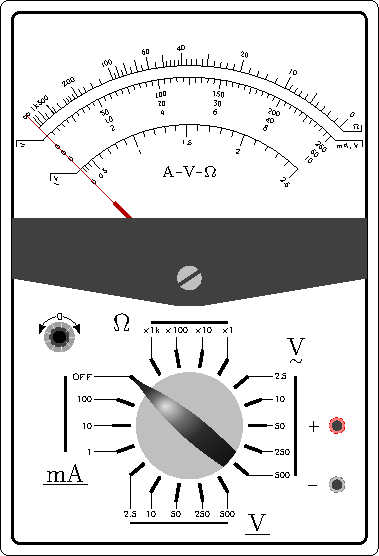
\includegraphics[scale=.75]{fig/9-10.png}
\caption{}
\end{figure}

在化纤、纺织等工业生产中,由于摩擦、分离等原因,织物
和纤维上常聚集有害的静电,将放射源放在容易产生静电的
地方,放射性物质放出的射线可以使空气分子电离变成导电
气体,这样可以把静电荷泄出.

用剂量不大的$\gamma$射线照射植物(棉花、白菜、萝卜等)的
种子能使产量显著增加.利用射线可以防治害虫,射线照射
能使幼虫失去发育能力,大剂量的照射能直接杀死害虫.射
线照射还能引起生物遗传特性发生突变以培育良种,在医疗
上射线可以使癌细胞受到抑制或死亡,因此常利用钴60的$\gamma$
射线来治疗肺癌、食道癌等.射线还可以消毒灭菌,处理医院
排除的污水,杀死各种病原体,保护环境卫生.

\subsection*{2.做为示踪原子}

放射性同位素跟同种元素的非放射
性位素的化学性质完全一样,如果在某种元素里搀进一些
放射性同位素,那么,无论这种元素走到哪里,它的放射性同
位素也经历同样的过程,由于放射性同位素会不停地放出放
射线,用适当的探测仪器探测这些放射线,就会知道这种元素
通过什么路径,运动到哪里了.人们把作这种用途的放射性
同位素叫做\textbf{示踪原子}.

示踪原子的应用是多方面的.在内燃机工作时,活塞上
的活塞环由于摩擦而磨损;如果使用带有放射性同位素铁59
的活塞环,这时具有放射性的铁59被磨掉而混入润滑油中,
测出油中的放射性就可以了解活塞环的磨损情况,而不必拆
开内燃机去检查.在农业施肥中,在肥料中加一些放射性同
位素,就会知道哪种农作物在什么季节最能吸收含哪种元素
的肥料.

在生物科学研究方面,同位素示踪技术也起着十分重要
的作用,我国科学家首先用人工方法合成了牛胰岛素,这是
我国科学战线上的一项重大成就,在这项工作中需要证明人
工合成的牛胰岛素结晶跟天然牛胰岛素的结晶是同一种物
质,因此,在合成过程中搀入放射性碳14作示踪原子,然后
把用碳14标记的人工合成的牛胰岛素与天然牛胰岛素混合
到一起,经过多次重新结晶后,得到了放射性碳14分布均匀
的牛胰岛素结晶,这就证明了人工合成的牛胰岛素与天然牛
胰岛素完全融为一体,它们是同一种物质,从而为我国在国际
上首先合成牛胰岛素提供了有力的证据.

放射线对人体组织是有伤害作用的,在使用放射性同位
素时必须注意安全,要防止放射性物质对水源、空气、用具、
工作场所的污染,并且要防止射线过多地照射人体.


\subsection*{练习二}

\begin{enumerate}
    \item 用$\alpha$粒子轰击氮核使它发生转变.从云室的照片中
    为什么可以确定细而长的径迹是质子产生的,粗而短的径迹
    是反冲氧核产生的.
    \item 用$\alpha$粒子轰击氩40,复核衰变时产生一个中子和一
    个反冲核,这反冲核是什么?写出核反应方程.
    \item 用$\alpha$粒子轰击硼10,产生一个中子和一个具有放射
    性的核,它是什么?这个核能放出正电子,它衰变后变成什
    么?写出核反应方程.
    \item 用中子轰击氮14,产生碳14,碳14具有$\beta$放射性,
    它放出一个$\beta$粒子后衰变成什么?写出核反应方程.
    \item 用中子轰击铝27,产生钠24,写出核反应方程.钠
    24是具有放射性的,衰变后变成镁24,写出核反应方程.
    \item 带电的验电器在放射线照射下电荷会很快消失,说
    明原因.
\end{enumerate}


\section{原子核的结合能}
\subsection{核力} 

原子核的半径很小,其中的质子之间的库仑斥力
是很大的,然而通常的原子核却是很稳定的.这表明,在原
子核里,除了质子间的库仑力,还有另一种力,它把各种核子
紧紧地拉在一起.这种力叫做\textbf{核力}.从实验知道,核力是一
种很强的力,它在质子和质子间、质子和中子间、中子和中子
间都存在,并且只在$2.0\x10^{-15}$米的短距离内起作用,超过
了这个距离,核力就迅速减小到零,质子和中子的半径大约
是$0.8\x10^{-15}$米,因此每个核子(质子或中子)只跟它相邻的
核子间才有核力的作用.核力只在很短的距离内发生作用,
因此它既不是电磁力,也不是万有引力.关于核力的本质问
题现在仍在深入研究中.

\subsection{结合能}

由于核子间存在强大的核力,所以原子核是
一个坚固的集合体,要把原子核拆散成核子,需要克服核力
做巨大的功,或者说需要巨大的能量.例如,用强大的$\gamma$光
子照射氘核(它是由1个质子和一个中子组成的),可以使它
分解为质子和中子,这时的核反应方程是:
\[\gamma +\atom{H}{2}{1}\longrightarrow \atom{H}{1}{1}+\atom{n}{1}{0} \]
从实验知道,当光子能量小于2.22MeV时,这个反应并
不发生;只有光子的能量等于或大于2.22MeV时,这个
反应才会发生.相反的过程,例如一个中子和一个质子结合
成氘核,要放出2.22MeV的能量,这个能量以$\gamma$光子的
形式辐射出去.这时的核反应方程是:
\[\atom{n}{1}{0}+ \atom{H}{1}{1}\longrightarrow \atom{H}{2}{1} +\gamma  \]

这表明,核子结合成原子核时要放出一定的能量;原子核
分解成核子时,要吸收同样多的能量.这个能量叫做原子核
的\textbf{结合能}.

\subsection{质能方程~~质量亏损}

怎样才能求出原子核的结合能
呢?虽然核力的本质还在研究之中,但是物理学家却有办法
求出结合能.这要归功于大科学家爱因斯坦,他从相对论得
出质量和能量间有下述关系:
\[E=mc^2\]
这个方程叫做爱因斯坦质能联系方程,简称\textbf{质能方程},式中$c$
是真空中的光速,$m$是物体的质量,$E$是物体的能量,这个方
程表明,物体的质量跟它的能量有一定的联系:物体的能量
跟它的质量成正比,如果物体的能量增加了$\Delta E$,物体的质量
也相应地增加$\Delta m$,反过来也一样.$\Delta E$和$\Delta m$之间的关系符
合爱因斯坦的质能方程
\[\Delta E=\Delta m\cdot c^2\]

核子结合成原子核时要放出结合能,原子核的能量要比
组成核的核子的能量小,所以原子核的质量也要比组成核的
核子的质量小.我们把组成原子核的核子的质量与原子核的
质量之差叫做核的质量亏损.如果知道核的质量亏损,根据
质能方程就可以求出核的结合能.

例如,氦核是由2个质子和2个中子组成的.每个质子
的质量$m_p$是1.007277u,每个中子的质量$m_n$是1.008665u.氦
核的质量$m_{\alpha}$是4.001509u.这里u表示原子质量单位,$1u=
1.660566\x10^{-27}{\rm kg}$.氦核的质量亏损$\Delta m$可以计算如下:
\[\begin{split}
    2m_p&=2\x1.007277{\rm u}=2.014554{\rm u}\\
    2m_n&=2\x1.008665{\rm u}=2.017330{\rm u}\\
    m_{\alpha}&=4.001509{\rm u}\\
    Δm&=2m_p+2m_n-m_{\alpha}=0.030375{\rm u}\\
\end{split}\]

在原子核物理学中,核的结合能是用MeV来表示的.
按照$E=mc^2$可以求出,$1u=931.5{\rm MeV}$.因此氦核的结
合能是
\[0.030375\x 931.5{\rm MeV}=28.3{\rm MeV}\]

\subsection{平均结合能} 

如果用核子数去除核的结合能,就得到每
个核子的平均结合能.对于氦来说,就是$28.3{\rm MeV}/4=
7.1{\rm MeV}$.用同样的方法,可以求出其他原子核中每个核
子的平均结合能,平均结合能是核子结合成原子核时每个核
子平均放出的能量,也是把原子核分解成核子时每个核子平
均吸收的能量.平均结合能越大,原子核就越难拆开.可见
平均结合能的大小能够反映核的稳定程度.图9.11表示核
子的平均结合能随原子核的质量数的变化规律.图中的横坐
标表示核的质量数,纵坐标表示核子的平均结合能.从图中
可以看出,质量数较小的轻核和质量数较大的重核,平均结合
能都比较小,中等质量数的原子核,平均结合能大.质量数
为50—60的原子核,平均结合能最大,约为8.6MeV.

\begin{figure}[htp]
\centering
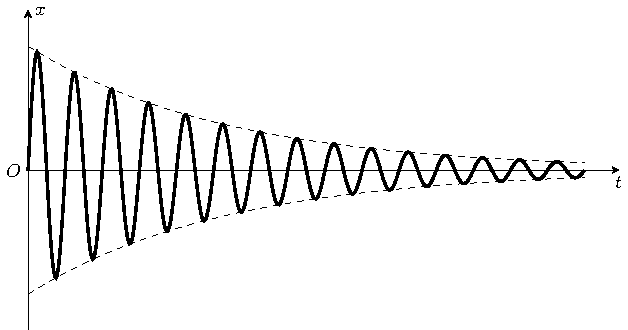
\includegraphics[scale=1.3]{fig/9-11.pdf}
\caption{平均结合能曲线}
\end{figure}


\subsection*{练习三}

\begin{enumerate}
    \item 氘核的质量是2.013553u,根据质量亏损,计算氘核的结合能.
    \item 碳原子的质量是12.000000u,可以看做是由6个氢
原子(质量是1.007825u)和6个中子组成的.求碳原子核的
结合能.(在计算中可以用碳原子的质量代替碳原子核的质
量,用氢原子的质量代替质子的质量,因为电子的质量可以在
相减过程中消去.)
\item  在$\atom{He}{4}{2}$,$\atom{Kr}{82}{36}$,$\atom{U}{238}{92}$等原子核中核子的平均结合能个最大?哪个最小?原子核的结合能哪个最大?哪个最小?(根据平均结合能曲线进行比较)
\item 如果要把$\atom{O}{16}{8}$分成8个质子和8个中子,要给它多
少能量?要把它分成$\atom{He}{4}{2}$,要给它多少能量?已知$\atom{O}{16}{8}$的核
子平均结合能是7.98MeV,$\atom{He}{4}{2}$的核子平均结合能是
7.07MeV.
\item 在一次核反应中,铀核$\atom{U}{235}{92}$变成了氙核$\atom{Xe}{136}{54}$和锶
核$\atom{Sr}{90}{38}$(同时放出了若干中子).铀核的核子平均结合能约为
7.6MeV,氙核的核子平均结合能约为8.4MeV,锶核
的核子平均结合能约为8.7MeV.
\begin{enumerate}
    \item 把U235分解为核子,要吸收多少能量?
    \item 再使相应的核子分别结合成Xe136和Sr90,要放出多少能量?
    \item 在这个核反应中是吸收还是放出能量?这个能量大
约是多大?
\end{enumerate}
\end{enumerate}


\section{重核的裂变}
重核的核子平均结合能比中等质量的核的核子平均结合
能小.因此,重核分裂成中等质量的核时,会有一部分结合能
释放出来.这是释放原子核能——原子能的一种重要方法.
这种核反应叫做\textbf{裂变}.

\subsection{铀核的裂变}

重核的裂变是在本世纪三十年代末期用中
子轰击铀核时发现的.铀核裂变的产物是多种多样的,有时裂
变为氙(Xe)和锶(Sr),有时裂变为钡(Ba)和氮(Kr)或锑(Sb)
和铌(Nb),同时放出2—3个中子,铀核还可能分裂成三部分
或四部分,不过这种情形比较少见.

铀核的裂变过程,可以用下面的示意图来说明(图9.12).
\begin{figure}[htp]\centering
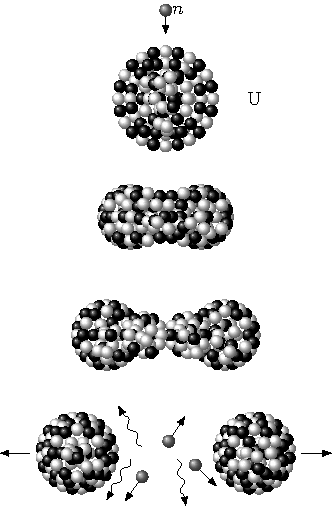
\includegraphics[scale=.75]{fig/9-12.png}
\caption{}
\end{figure}

当中子打进铀235后,就
形成处于激发状态的复核,复
核中的核子由于激烈运动,使
核变成不规则形状,核子间的
距离增大.由于核力只在极短
距离内发生作用,当核子间距
离增大时,核力迅速减小,因而
不能克服质子间的库仑斥力使
核恢复原状,核就分裂成两部
分,同时放出几个中子.

轴核裂变的许多可能的核
反应中的一个是:
\[\atom{U}{235}{92}+\atom{n}{1}{0}\longleftarrow \atom{Ba}{141}{56}+\atom{Kr}{92}{36}+3\atom{n}{1}{0}\]
在这个反应中释放的能量可以计算如下:
裂变以前:
\[235.0439{\rm u}+1.0087{\rm u}=236.0526{\rm u} \]
裂变以后:
\[140.9139{\rm u}+91.8973{\rm u}+3.0261{\rm u}=235.8373{\rm u} \]
反应过程中质量减少$\Delta m=0.2153{\rm u}$,反应中释放的能量
\[\Delta E=\Delta m\cdot c^2=201{\rm MeV}\]
在不同的反应中,铀核释放的能量也不同.如果按照一个铀
核裂变时放出200MeV的能量来估算,1千克铀全部裂
变时放出的原子能就相当于2500吨优质煤完全燃烧时放出
的化学能.

\subsection{链式反应} 

铀核裂变时,同时放出2—3个中子,如果这
些中子再引起其他铀核裂变,就可使裂变反应不断地进行下
去,这种反应叫做链式反应(图9.13).

\begin{figure}[htp]
    \centering
    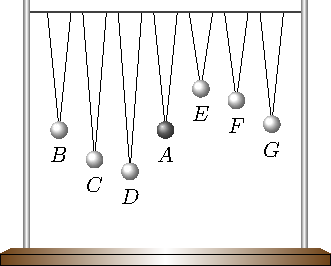
\includegraphics[scale=.7]{fig/9-13.pdf}
    \caption{链式反应}
\end{figure}


在天然铀中,主要有两种同位素,其中99.3\%是铀238,
0.7\%是铀235.这两种铀跟中子的作用很不相同.铀235俘
获各种能量的中子都会发生裂变,而且俘获能量低的中子发
生裂变的几率较大,铀238只有俘获能量大于1MeV的
中子才可能发生裂变,并且几率很小,它俘获能量低于1MeV的中子时不发生裂变,而变成铀239.能量低于1eV的中子跟铀238基本上只发生弹性碰撞,不引起核反应.因
此,为了使裂变的链式反应容易发生,最好是利用纯铀235.

铀块的体积对于产生链式反应也是一个重要因素.因为
原子核非常小,如果铀块的体积不够大,中子从铀块中通过
时,可能还没有碰到铀核就跑到铀块外面去了,能够发生链
式反应的铀块的最小体积叫做它的临界体积.

如果铀235的体积超过了它的临界体积,只要有中子进
入铀块,会立即引起铀核的链式反应,在极短时间内就会释放
出大量的核能,发生猛烈的爆炸,原子弹就是根据这个原理
制成的.

\subsection{核反应堆}

核反应堆是用人工控制链式反应的装置.原
子弹爆炸时链式反应的速度是无法控制的,为了用人工方法
控制链式反应的速度,使核能比较平缓地释放出来,人们制成
了核反应堆.
\begin{figure}[htp]
    \centering
    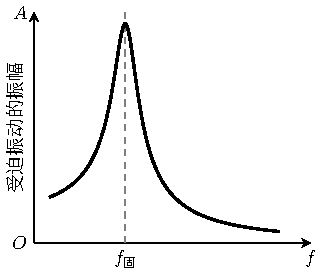
\includegraphics[scale=1.2]{fig/9-14.pdf}
    \caption{原子反应堆示意图}
\end{figure}

图9.14是原子反应堆的示意图,反应堆里用的铀棒是天
然铀或浓缩铀(其中铀235的含量比天然铀高),由于裂变产
生的是速度很大的快中子,很容易被铀238俘获而不发生裂
变,所以必须设法使中子在碰上铀238前降低速度.为此在
铀棒的周围放上原子量比较小、又不吸收或很少吸收中子的
物质,如石墨、重水或普通水(普通水吸收中子的几率较大,但
可用在用浓缩铀做原料的反应堆中),快中子跟这些物质的原
子核碰撞后,能量减小,变成慢中子.这种用来使中子减速的
物质叫做\textbf{减速剂}.速度跟热运动速度差不多的慢中子(能量约
为1/40电子伏)叫做热中子.热中子碰到铀238时会弹射回
来,却容易被铀235俘获而引起裂变,为了调节中子数目以
控制反应速度,还需要在铀棒之间插进一些镉棒,镉吸收中
子的能力很强,当反应过于激烈时,使镉棒插入深一些,让它
多吸收一些中子,链式反应的速度就会慢一些;当反应过于缓
慢,达不到所需功率时,使镉棒插入浅一些,让它少吸收一些
中子,链式反应速度就可以增大,这种镉棒叫做\textbf{控制棒}.用电
子仪器自动地调节控制棒的升降,就能使反应堆保持一定的
功率安全地工作.

反应堆工作时,核燃料裂变释放出的核能转变为热能,使
反应堆的温度升高,为了控制反应堆的温度,使它能正常工
作,需要用水、液体金属钠或空气等流体作冷却剂,在反应堆
内外循环流动,不断地带走热能.这就是反应堆的冷却系统,
它同时可以用来输出热能.

为了防止铀核裂变物放出的各种射线对人体的危害,在
反应堆的外面需要修建很厚的水泥防护层,用来屏蔽射线,不
让它们透射出来,对放射性的废料,也要装入特制的容器,埋
入深地层进行处理.

利用反应堆工作时释放出的热能使水汽化以推动汽轮发
电机发电,这就是核电站.图9.15是核电站示意图.核电站
消耗的“燃料”很少.一座一百万千瓦的核电站,每年只消耗
30吨浓缩铀,而同样功率的火力发电站,每年却要消耗250万
吨煤.目前,核能发电的经济效益跟火电站大体相同,到1983
年底、核发电已占世界发电总量的12\%.为了适应我国现代
化建设对能源日益增长的需要,在广东、浙江、江苏、辽宁等省
正在建造核电站.

\begin{figure}[htp]
    \centering
    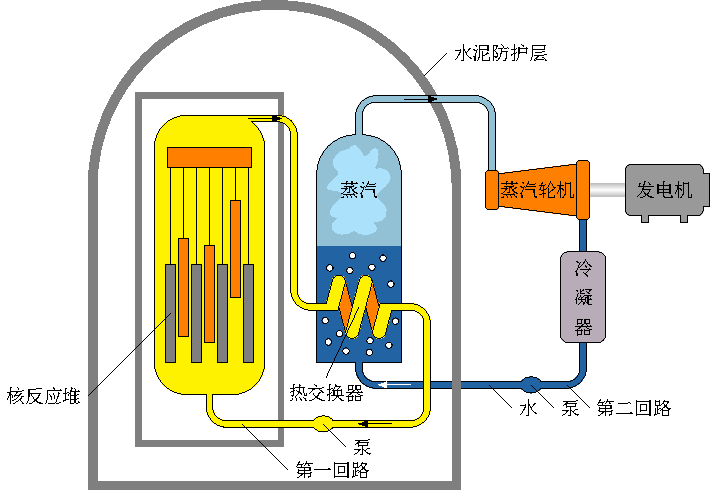
\includegraphics[scale=.8]{fig/9-15.pdf}
    \caption{核电站示意图}
\end{figure}

原子能反应堆不仅可以提供强大的原子能,而且它产生
的大量中子还可以用来进行各种原子核物理实验,制造各种
放射性同位素.

利用原子能反应堆还可以生产新的核燃料,从实验知道,
快中子被铀238俘获后,变成铀239,铀239是不稳定的,经过
两次$\beta$衰变后变成钚239.钍232与中子作用后,经过两次$\beta$
衰变后变成铀233,钚239和铀233的性质跟铀235一样,很
容易俘获中子而发生裂变,因此也可以作为供裂变用的核燃
料.因此,如果在反应堆中装入铀238或钍232,并设法使每
一次核裂变能够产生一个以上的钚239或铀233,那么,我们
就可以使新产生的核燃料多于消耗的核燃料,使铀238和钍
232也可以得到利用,这种反应堆叫做增殖反应堆,地球上
的铀238和钍232的总量大约是铀235的800倍,建造增殖
反应堆可以利用铀238和钍232,更有效地利用核资源.增
殖反应堆虽然处于试验阶段,但从长远来看是很有前途的.

\section{轻核的聚变}
\subsection{聚变}
轻核的结合能更小,某些轻核结合成质量较大的
核时,能释放出更多的结合能.例如:一个氘核和一个氚核结
合成一个氨核时,释放出17.6MeV的能量,平均每个核
子放出的能量在3MeV以上,这时的核反应方程是
\[\atom{H}{2}{1}+\atom{H}{3}{1}\longrightarrow \atom{He}{4}{2}+\atom{n}{1}{0} 
    \]
轻核结合成质量较大的核叫做\textbf{聚变}.

使核发生聚变,必须使它们接近到$10^{-15}$米,也就是接近
到核力能够发生作用的范围.由于原子核都是带正电的,要
使它们接近到这种程度,必须克服电荷之间的很大的斥力作
用.这就要使核具有很大的动能.用什么办法能使大量的轻
核获得足够的动能来产生聚变呢?有一种办法,就是把它们
加热到很高的温度.从理论分析知道,物质达到几百万度以
上的高温时,原子的核外电子已经完全和原子脱离,这时小部
分原子核就具有足够的动能,能够克服相互间的库仑斥力,在
互相碰撞中接近到可以发生聚变的程度.因此,这种反应又
叫做热核反应,怎样产生这样高的温度呢?我们知道,原子
弹爆炸时能产生这样高的温度,所以可以用原子弹来引起热
核反应,氢弹就是这样制造出来的.

热核反应在宇宙中是很普遍的现象.在太阳内部和许多
恒星内部,温度都高达1千万度以上,在那里热核反应激烈地
进行着,太阳每秒钟辐射出来的能量约为$3.8\x10^{26}$焦,就是
从热核反应中产生的,地球只接受了其中的二十亿分之一,就
使地面温暖,产生风云雨露,河川流动,生物生长.

\subsection{可控热核反应}

原子弹、氢弹虽然能够引起热核反应释
放出巨大能量,但能量是瞬时释放出来的.和平利用核能则
需要聚变能缓慢而稳定的释放,释放的速率应当能够被人控
制,即发生可控热核反应,这种反应就是用人工的办法,有控
制地使氘核产生聚变反应,从而释放出能量.热核反应需要的
原料——氘,在世界上的储量是非常丰富的.1升海水中大约
有0.03克的氘,如果用来发生热核反应,它放出的能量就和
燃烧三百升汽油相当,因此海水中的氘就是异常丰富的能源.

热核反应除了原料丰富外,还有以下几个特点:它释放
出的能量,就每一个核子平均来说,比裂变反应要大好几倍.
而且裂变反应会产生带有强放射性的物质,对环境造成放射
性污染;热核反应对环境的污染要轻得多,也比较容易处理.
从热核反应中还可以得到大量有用的中子.可控热核反应是
核能利用的一条途径,受到普遍重视.

目前,世界上许多国家,都在积极研究可控热核反应的理
论和技术.我国自行设计和制造的可控核聚变实验装置“中
国环流器一号”已于1984年9月顺利启动,它标志着我国研
究可控热核聚变的实验手段有了新的发展和提高,必将为人
类探求新能源作出贡献.

\section{基本粒子}

直到十九世纪末,人们都认为原子是组成物质的最小的
不可再分的微粒,后来发现了电子、质子和中子,并且知道了
质子和中子组成了原子核,原子核和电子组成了原子,这时
许多人又认为电子、质子和中子是组成物质的最基本的粒子,
把它们叫做\textbf{基本粒子}.

随着科学技术的发展,从二十世纪三十年代以来,人们不
断地从宇宙射线和原子核物理实验中发现了大量的基本粒
子.

宇宙射线是从宇宙空间射来的高能粒子,其中主要是质
子,还有少量的$\alpha$粒子和其他粒子.这些粒子的能量很高,大
部分高达$10^9$—$10^{10}$eV,少数粒子具有更高的能量,宇宙
射线进入地球大气层后,跟大气中的原子核碰撞,会引起很多
种核反应,产生各种核反应产物,自从1911年发现宇宙射线
以后,就开始了对宇宙射线的观测,在宇宙射线的研究中,陆
续发现了一些新的基本粒子:1932年发现正电子,1937年发
现$\mu$介子(后来称为$\mu$子),1947年又发现K介子和$\pi$介子.
这些介子的质量是介于质子和电子之间的,因此叫做介子,后
来又发现了质量比质子大的粒子,名叫\textbf{超子}\footnote{六十年代以后,又发现了质量比质子大的介子,因此介子、超
子这些名称只具有历史上的意义.}.

1932年发明了回旋加速器,后来建成了各种加速器.在
用加速器进行的实验中,发现了更多的基本粒子.并且发现,
许多粒子都有和它的质量相同而电荷相反的粒子,叫做\textbf{反粒
子}.例如,电子的反粒子就是正电子,正$\pi$介子的反粒子就是
负$\pi$介子,质子的反粒子叫做反质子,是1955年发现的,它带
有单位负电荷,现在发现的基本粒子已达几百种.

按照基本粒子之间的相互作用,可以把它们分为三类:

1. \textbf{强子:} 核子之间的核力是一种比电磁作用大得多的
相互作用,叫做\textbf{强相互作用}.凡是参与强相互作用的粒子,都
叫做强子,目前发现的基本粒子,绝大多数是强子,质子是最
早发现的强子,强子又分重子(中子、质子、超子)和介子两类.

2. \textbf{轻子:} 都不参与强相互作用,只发现几种.电子是最
早发现的轻子.$\mu$子从它的许多性质来看属于轻子,1975年,
又发现了一种质量很大的轻子,称为$\tau$子,也叫重轻子.

3. \textbf{媒介子:} 是传递粒子间相互作用的粒子,例如光子就
是其中的一种,是传递电磁相互作用的.

绝大多数基本粒子都是不稳定的,在很短时间内就发生
衰变,并且能相互转变,例如,正负$\pi$介子的平均寿命约为
$2.6\x10^{-8}$秒,它衰变为$\mu$子,同时产生一种质量非常小(与电
子质量相比,可以认为质量为零)的中性粒子,叫做\textbf{中微子},它
属于轻子,用$\nu$表示.$\mu$子也是不稳定的,平均寿命约为$2.2\x
10^{-8}$秒,衰变为电子和正反两个中微子.

中子也可以转化,自由状态的中子的平均寿命约为16分,
它衰变为一个质子、一个电子和一个反中微子;
\[\atom{n}{1}{0}\longrightarrow \atom{p}{1}{1}+\atom{e}{0}{-1}+\nu   \]
放射性原子核的$\beta$衰变,实际发生的就是这种反应,由中子转
化成的质子仍留在原子核内,同时产生的电子(即$\beta$粒子)和
反中微子则放射出去.

质子在自由状态是稳定的,但在原子核内也会转化为一
个中子,同时放出一个正电子和一个中微子:
\[\atom{p}{1}{1}\longrightarrow \atom{n}{1}{0}+\atom{e}{0}{1}+\nu   \]
放射性同位素磷30的衰变,实际发生的就是这种反应.

一对正反粒子相遇时,会同时消失而转化为别种粒子,这
种现象叫做\textbf{湮灭},例如,一个电子和一个正电子相遇会发生
湮灭而转化为一对光子:
\[\atom{e}{0}{-1}+\atom{e}{0}{1}\longrightarrow \gamma+\gamma  \]

相反的过程也能够发生.例如,能量超过1.02MeV
的$\gamma$光子穿过铅板时,会同时产生电子和正电子,通常把这一
对正负电子叫做电子-正电子偶.图9.16是在云室中看到的
它们的径迹,由于电子和正电子所带的电荷相反,它们在磁场
中向相反的方向偏转,这个反应可表示为:
\[\gamma\longrightarrow \atom{e}{0}{-1}+\atom{e}{0}{1} \]
这些事实表明,光子和电子虽然有基本的区别,但是仍然有着
深刻的联系.
\begin{figure}[htp]\centering
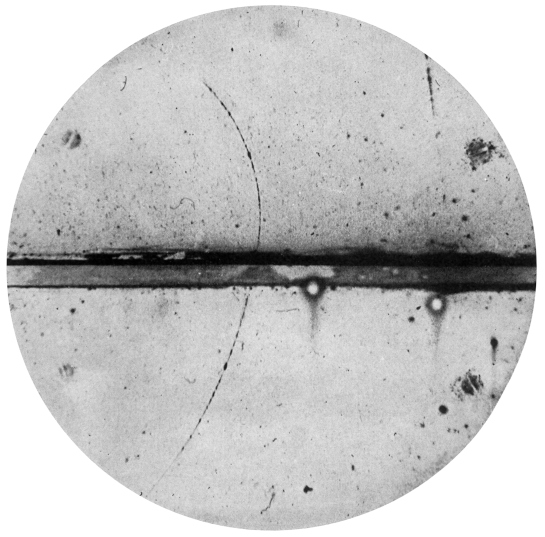
\includegraphics[scale=.75]{fig/9-16.png}
\caption{电子-正电子偶的径迹}
\end{figure}



基本粒子的种类这样多,并且能够相互转化,这就促使人
们进一步去研究基本粒子的结构.许多实验事实表明,强子
是有内部结构的,因此许多物理学家倾向于不再使用“基本
粒子”这个名称,而改称为“粒子”.为了探索强子的内部结构,
先后提出了多种模型,其中比较成功的是\textbf{夸克模型},认为强子
是由夸克(我国也叫层子)组成的.目前,这个模型里有六类
(共十八种)夸克,还有同样数目的反夸克,它们所带的电荷是
基本电荷的$\pm1/3$或$\pm 2/3$.
重子是由三个夸克组成的,反重子
是由三个反夸克组成的,介子是由一个夸克和一个反夸克组
成的.从夸克理论得出的许多结果都跟实验符合得很好,但
在实验中还没有发现自由夸克.关于夸克模型的理论正在进
一步发展中.

物质世界,无论从宏观方面看,还是从微观方面看,都是
无穷尽的,人类对物质世界的认识将一步一步地深人,永远不
会终止.关于基本粒子的物理学——高能物理正在蓬勃发展
中,人们终将认识基本粒子的结构和变化规律.


\section*{复习题}
\begin{enumerate}
    \item 什么是放射性元素?$\alpha$射线、$\beta$射线、$\gamma$射线的本质是什么?三种射线各有什么特性?

    什么是$\alpha$衰变?$\alpha$衰变的规律是什么?什么是$\beta$衰变?$\beta$
    衰变的规律是什么?什么是半衰期?
    \item 说明用云室、计数器、乳胶照相探测射线的基本原
    理.
    \item 什么是质子?质子是怎样发现的?什么是中子?中子
    是怎样发现的?原子核是怎样组成的?什么是同位素?
    \item 简述放射性同位素有哪些应用.
    \item 什么是原子核的结合能?什么是爱因斯坦的质能方
    程?怎样根据质能方程计算结合能?什么是平均结合能?平均
    结合能的大小反映核的什么性质?
    \item 什么是重核的裂变?什么是链式反应?在核反应堆中
    怎样控制裂变的速度?
    \item 什么是轻核的聚变?产生聚变的条件是什么?研究
    可控热核反应有什么意义?
    \item 简述基本粒子的种类.
\end{enumerate}


\section*{习题}
\begin{enumerate}
    \item 铀238的半衰期是$4.5\x 10^9$年,假设一块矿石中含
有1千克的铀238,经过45亿年(相当于地球的年龄)以后,
还剩有多少铀238?假设发生衰变的铀238都变成了铅206,
矿石中会有多少铅?这时铀铅的比例是多少?再经过45亿年,
矿石中的铀铅比例将变成多少? 根据这种铀铅比例能不能判
断出矿石的年龄?
\item 镭核在$\alpha$衰变中放出能量为4.78MeV的$\alpha$粒
子和能量为0.19MeV的$\gamma$粒子.如果1克镭每秒钟有
$3.7\x10^{10}$个原子核发生$\alpha$衰变,算出它每秒钟释放多少能量.
\item 静止状态的放射性原子核镭($\atom{Ra}{226}{88}$)进行$\alpha$衰变.为
了测量$\alpha$粒子的动能$E$,让$\alpha$粒子垂直飞进$B=1$特的匀强磁
场,测得$\alpha$粒子的轨道半径$r=0.2$米.
\begin{enumerate}
    \item 写出Ra的$\alpha$衰变方程.
    \item 试计算$\alpha$粒子的动能$E$.
\end{enumerate}

\item 在某些恒星内,三个$\alpha$粒子结合成一个$\atom{C}{12}{6}$核.$\atom{C}{12}{6}$
的质量是12.0000u,$\atom{He}{4}{2}$的质量是4.0026u.这个反应中放出
多少能量?
\item 已知$\atom{Ra}{226}{88}$,$\atom{Rn}{222}{86}$,$\atom{He}{4}{2}$的原子量分别是226.0254,
222.0175,4.0026.求在$\atom{Ra}{226}{88}$衰变
\[\atom{Ra}{226}{88}\longrightarrow \atom{Rn}{222}{86}+\atom{He}{4}{2}\]
中放出的能量是多少电子伏?如果这些能量都以Rn核和He
核的动能形式释放出来,放出的$\alpha$粒子的速度有多大?

提示:能量和动量都守恒.

\item 在一原子反应堆中,用石墨(碳)作减速剂使快中子
减速.已知碳核的质量是中子的12倍,假设把中子与碳核的
每次碰撞都看作是弹性正碰,而且认为碰撞前碳核都是静止
的.
\begin{enumerate}
    \item 设碰撞前中子的动能是$E_0$,经过一次碰撞,中子损失的能量是多少?
    \item 至少经过多少次碰撞,中子的动能才能小于$10^{-6}E_0$?
\end{enumerate}

\end{enumerate}


































